\chapter{Implementation in das Dietrich Projekt}

In diesem Kapitel wird die Implementation ins Dietrich-Projekt genauer erläutert.

\section{Vorbereitung}

Zuerst muss der ElasticSearch Client bei Composer hinzugefügt werden. Danach ist der PHP-Client nutzbar. 

Um für die Vergleiche ein faires Spielfeld zu bauen, wurde dieselbe MYSQL-Datenbank verwendet. Diese Datenbank liegt auf denselben Server wie ElasticSearch. Das bedeutet, dass Doctrine nun zu demselben Server kommuniziert wie der PHP-Client von ElasticSearch.

Zum Testen wird nun zuerst der Lemma-Query, in einer modifizierten Fassung \ref{lemmaIndexierungEla}, verwendet, der auch schon bei dem vorherigen Vergleich hinhalten musste.

Um den ElasticSearch-Client zu verwenden, muss zuerst ein API-Key generiert werden \ref{lst:elaApi}. Dabei bekommt der API-Key lesende Rechte für alle Indices mit dietrich-Präfix. 

\begin{lstlisting}[language=XML, frame=single, label={lst:elaApi}] 
    POST /_security/api_key
    {
      "name": "dietrich-webiste",
      "role_descriptors": { 
        "role-a": {
          "cluster": ["all"],
          "index": [
            {
              "names": ["dietrich_*"],
              "privileges": ["read"]
            }
          ]
    }}}
\end{lstlisting}

Zudem muss auch wieder die CA für den Aufbau der SSL-Verbindung genutzt werden.


\subsubsection{Indexierung}
\label{lemmaIndexierungEla}

Um nun alle Daten in richtiger Form in das Projekt zu laden, muss die Indexierung von damals umgeschrieben werden. 

Bei den Joins wurden m zu n Beziehungen auf eine flache Ebene gezogen. Dabei wird der Eintrag so oft abgebildet, wie es Objekte in der M zu N Beziehung gibt. 

Zur Verdeutlichung hier ein Beispiel.
Es gibt eine Tabelle Artikel, welche eine M zu N Beziehung mit der Tabelle DDC bezieht. In der Artike Tabelle gibt es den Eintrag Trier mit der ID 1, der mit 2 DDC Einträgen, Trier und Rheinland-Pfalz verbunden wird. Bei einen Join wird nun alles in eine flache Hirachie gezogen. Deswegen würde die Tabelle der Ergebnisse des Joins nun die Folgenden Einträge enthalten \ref{tbl:join}.

\begin{table} %[hbtp]
	\centering
		\begin{tabular}{l | l | l}
		    \textbf{ID} & \textbf{Artikel} & \textbf{DDC} \\
        \hline
        01 & Trier & Trier \\
        01 & Trier & Rheinland-Pflaz  \\
		\end{tabular}
    \caption{Tabelle für ein Beispiel der Joins}
    \label{tbl:join}
\end{table}

Um nun einen solchen Eintrag in ElasticSearch abzubilden wäre es schön eine Art Array für die DDC Einträge zu haben. Für solche Fälle gibt es den Aggregat-Filter in Logstash. Dieser Aggregiert auf Basis der ID die Daten. So ist es nun möglich Code zu schreiben, der automatisch die Daten in Arrays zusammenfasst. Der Aggregat-Filter wird nun also so lange durchlaufen, wie dieselbe ID hintereinander aus der Datenbank kommt. 

Deswegen ist es wichtig, dass diese Prozess nicht in mehreren Threads ausgeführt wird. Daher erhalten alle Pipelines auch nur einen Thread in diesem Projekt.


\begin{lstlisting}[language=XML, frame=single, label={lst:fronendConf}] 
  [...]
  map['bstatus_beschreibung'] ||= event.get('bstatus_beschreibung')

  map['ddc_entries'] ||= []
  if event.get('ddc_notation') != nil
      duplicate = false
      map['ddc_entries'].each { |n|
          if n.value?(event.get('ddc_notation'))
             duplicate = true
             break
          end
      }
      if !duplicate
          map['ddc_entries'] << {
              'ddc_notation' => event.get('ddc_notation'),
              'ddc_schlagwort' => event.get('ddc_schlagwort'),
              'ddc_webdewey_is_checked' => 
                event.get('ddc_webdewey_is_checked')
          }
      end
  end
  [...]
\end{lstlisting}

Der Wert bstatus\_beschreibung wird nun bei jeden Durchlauf überschrieben. 

Um nun aber die sich ändernden Werte zu aggregieren, wurde ein Code geschrieben, welche die Einträge in eine Array schreibt \ref{lst:fronendConf}. Da hier nun allerdings mehr als eine Tabelle mit m zu n Beziehungen gejoint wird, ist es notwendig ein paar Überprüfungen auszuführen. Zum einen soll ein Wert nur aggregiert werden, wenn er auch existiert. Sonst sind später Null-Werte in ElasticSerach, die nicht gewünscht sind. Als nächstes kann es aufgrund der Join Struktur dazu kommen, dass Duplikate eingetragen werden. Dafür schaut eine Schleife immer kurz nach, ob schon ein Wert in dem Array steht, bevor es ihr nochmals hereinschreibt. 

\section{Aufbau des Queries}

Als SQL-Framework wurde Doctrine verwendet. Dieses bietet eine Abstaktion für SQL in Objekte. Im Hintergrund werden diese Objekte dann in SQL übersetzt und abgesendet. Der hier betrachtete Query wurde schonmal von Hand optimiert, da zuerst alle Ids der anzuzeigenden Lemmata gesucht werden, und erst im zweiten Schritt alle Joins auf den Daten ausgeführt werden.

Der ElasticSerach Query besteht allerdings nur aus einer Abfrage, da hier schon alle Daten auf eine flache Ebene gezogen wurden.

Verwendet wurde hier ein sogenannten Boolean-Query. Dieser enthält vier verschieden Untergruppierungen.

Zuerst einmal der Must-Teil. Alle hier Angegeben Parameter müssen in jeden Ergebnis vorhanden sein. Dies ist gleichzustellen mit einen booleschen AND. 

Als zweites der Must-Not-Teil. Dieser Teil ist den Must-Teil sehr ähnlich, allerdings sind die Parameter negiert.

Danach der Shoud-Teil. In diesem Teil muss nur einer der Parameter vorhanden sein. Dies ist zu vergleichen mit einem booleschen OR. 

Und zuletzt der Filter-Teil. Die gesetzten Filter sind auch Must-Befehle. Allerdings werden diese nicht bei der Gewichtung der Ergebnisse mit reingerechnet. Für diese Arbeit hat dies erstmal keinen Einfluss, da alle Ergebnisse alphabetisch sotiert werden. Daher ist der Query mit Must gleichzustellen. \cite{ElasticsearchB.V..17.12.2019}


\begin{lstlisting}[language=PHP, frame=single, label={lst:queryEla}] 
  //Create Client with basic Params
  $mustNotQueries = [];
  $filters        = [];
  $mustQueries    = [];

  if ($character === LemmaEntity::NOT_A_TO_Z_CHARACTER) {
      $mustQueries[] = ['regexp' => ['bezeichnung.keyword' => 
        ['value' => '@&~(^[a-zA-Z].+)', 'flags' => 'ALL']]];
        
      $filters[]     = ['term' => ['ist_geloescht' => false]];
  } elseif ($character === LemmaEntity::DELETED) {
      $filters[] = ['term' => ['ist_geloescht' => true]];
  } else {
      $mustQueries = ['prefix' => ['bezeichnung.keyword' => "$character"]];
      $filters[]   = ['term' => ['ist_geloescht' => false]];
  }

  switch ($filter) {
      case self::STATUS_FILTER_KLAR:
          $filters[] = ['term' => ['bstatusbezeichnung' => 'klar']];
          break;
      //[Other Filters]
  }

  $params['body']['query']['bool']['must']     = $mustQueries;
  $params['body']['query']['bool']['must_not'] = $mustNotQueries;
  $params['body']['query']['bool']['filter']   = $filters;

  return $client->search($params)['hits']['hits'];
  
\end{lstlisting}

In Zeile 14 ist hier zu sehen, dass anstelle der Wildcard-Querys \ref{lst:phpElastic} ein Prefix-Query verwendet wird. Dieser bietet eine sauberere Lösung zum Suchen von Wortanfängen.

\section{Vergleich}

Die oben Beschriebenen Querys wurde jetzt jeweils 100-Mal mit einen Timer laufen gelassen. 
Dafür wurden die Methodenaufrufe, welche die Querys genieren und ausführen mit dem Timer umschlossen. 

Bei dem Vergleich kamen die folgenden Durchschnittswerte zustande:
\begin{table} %[hbtp]
	\centering
		\begin{tabular}{l | l }
		    \textbf{System} & \textbf{Zeit} \\
        \hline
        MariaDB + Doctrine & 3.49 \\
        ElasticSearch      & 1.45  \\
		\end{tabular}
    \caption{Vergleich der Laufzeit zur Abfrage aller Daten für Buchstabe S der Lemma-Administration (15.846 Einträge)}
    \label{vlgTimeDBvsEla}
\end{table}

Dabei sieht man, dass ElasticSearch eine Reduktion der Zeit um 58,45 \% ermöglicht.

Der Query wurde auch noch in einer nachgebauten Produktionsumgebung ausgeführt. Daran erkennt man, dass die Query durchaus schneller agiert, allerdings dies im Gesamtkontext sich nicht merkbar schneller anfühlt. Da ElasticSearch mit 46,49 Sekunden durchaus schneller lädt als Doctrine mit 50,1 Sekunden, aber die Gesamtzeit aktuell immer noch sehr hoch ist.

\begin{figure}
	\centering
	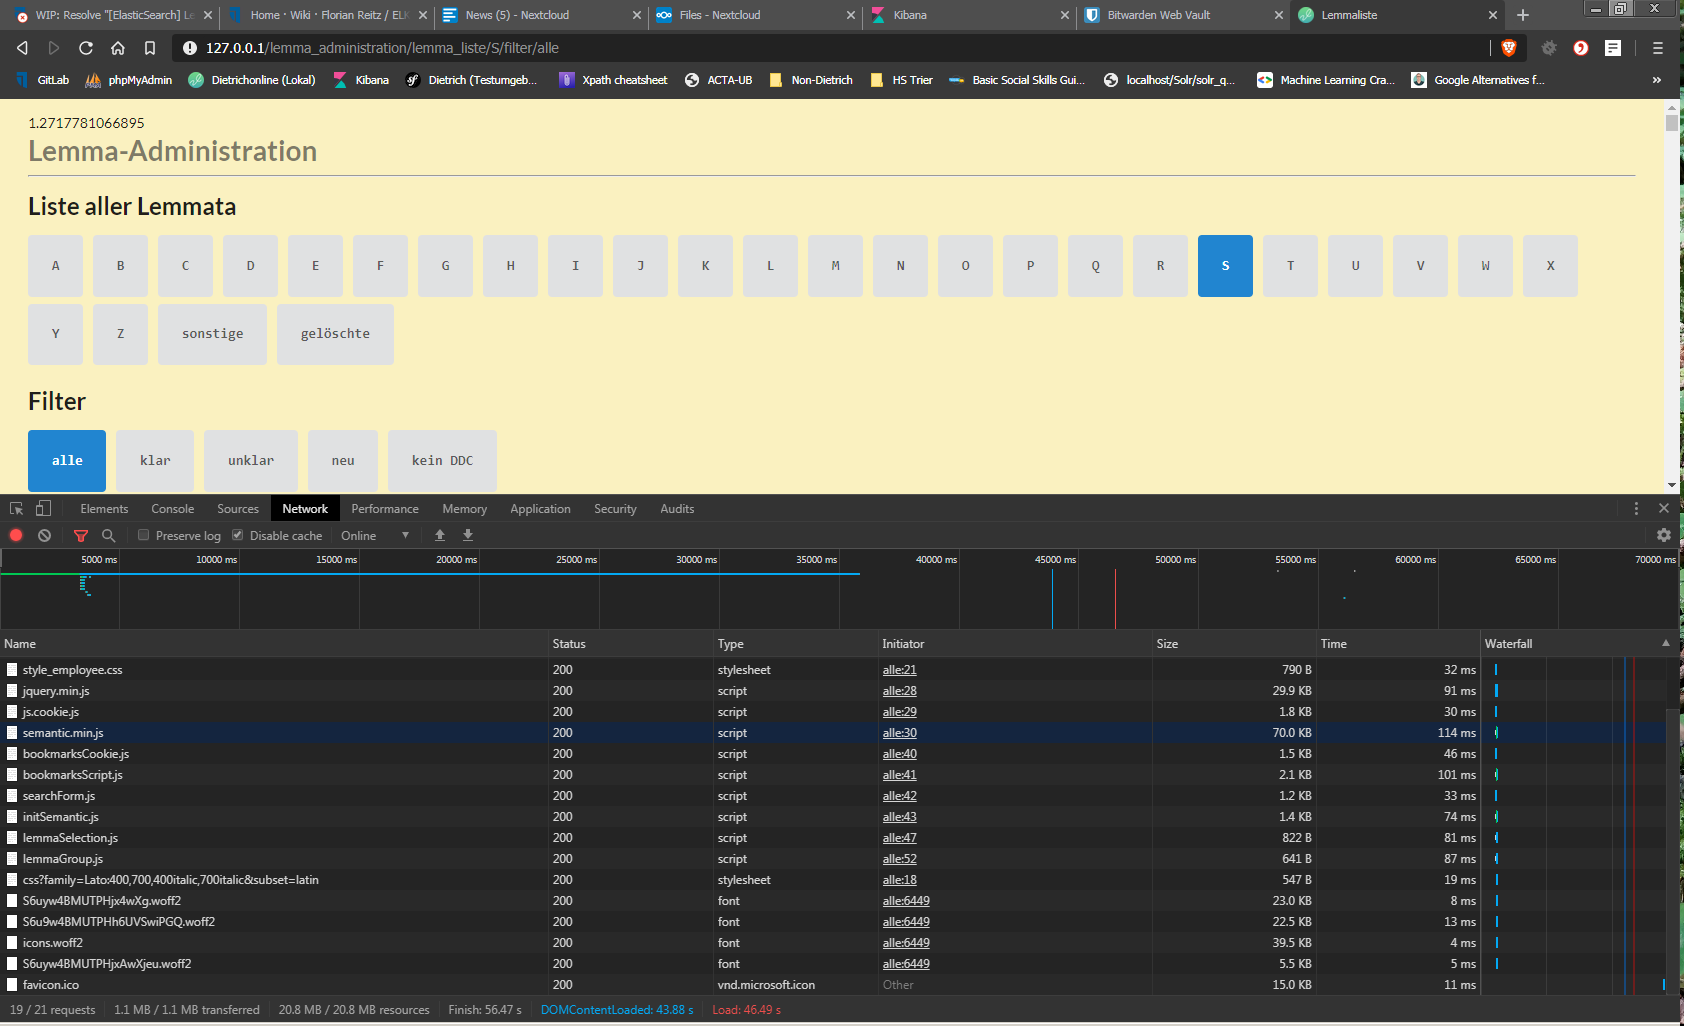
\includegraphics[width=1\linewidth]{images/setup/query/time_prod_ela.png}
	\caption{Query-Geschwindigkeit: ElasticSearch}
	\label{img:timeProdEla}
\end{figure}

\begin{figure}
	\centering
	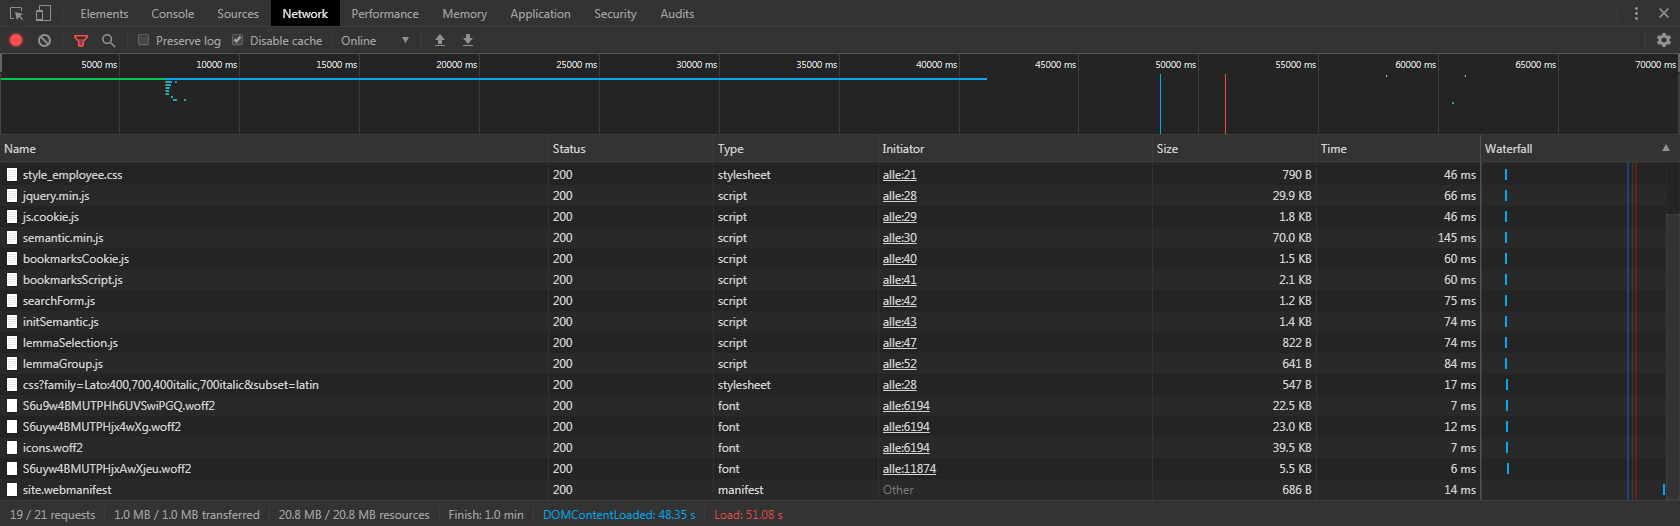
\includegraphics[width=1\linewidth]{images/setup/query/time_prod_db.png}
	\caption{Query-Geschwindigkeit: Doctrine+MySQL}
	\label{img:timeProdDb}
\end{figure}